\hypertarget{index_Introduction}{}\section{Introduction}\label{index_Introduction}
In the current R\+T\+E\+MS version, a lower-\/priority ready task must wait if all the processors included in its affinity mask are executing higher-\/priority tasks. Since a lower-\/priority task can never “dislodge” a higher-\/priority task that could also execute elsewhere, this may needlessly prevent some tasks from being scheduled, even if some processors idle as a result\mbox{[}1\mbox{]}.

This project aims to add the Strong Arbitrary Processor Affinity (Strong A\+PA) scheduler to $\ast$\+R\+T\+E\+MS. Strong A\+PA scheduler would allow higher-\/priority tasks to be ”dislodged” or moved among processors in order to make space for lower priority tasks that are limited by affinity constraints \mbox{[}1\mbox{]}. Consequently, this would allow R\+T\+E\+MS to achieve improved schedulability (i.\+e., lower response-\/time bounds).

There are two main scheduling events that affect the set of ready tasks\+: task arrival and task departure. The following example would show how when a task arrives, the scheduler tries to find a processor to task matching that has the lowest total sum of priorities of task scheduled than any other processor to task mapping (which means more higher priority task being scheduled). This is achieved by the newly arrived task searching for all the cpu\textquotesingle{}s in its affinity set, and further the already scheduled task searching in the cpu\textquotesingle{}s in their affinity set to find the minimum priority scheduled task and blocking it. The example below would help you understand this concept more clearly.

The task can be in following states\+:


\begin{DoxyImageNoCaption}
  \mbox{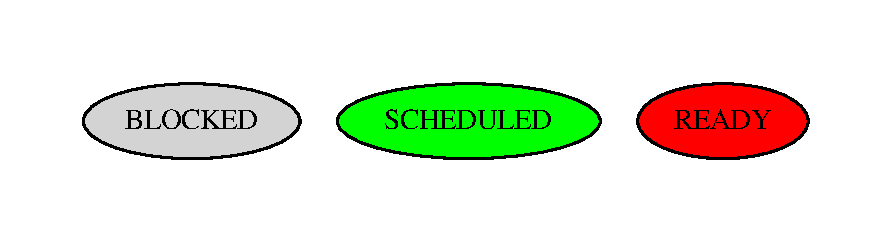
\includegraphics[width=\textwidth,height=\textheight/2,keepaspectratio=true]{dot_inline_dotgraph_1}}
\end{DoxyImageNoCaption}


Numbers in bracket indicate\textquotesingle{}s the task\textquotesingle{}s priority. A higher number means that the task has a lower priority. (Since we always allocate priority 0 to the most important or the highest priority tasks in R\+T\+O\+Ses).

System Description\+:

There are three processors (C\+P\+Us), C\+PU 0,1 and 2. The system has 4 tasks.

Task A has priority 1 and has affinities to C\+PU 1 and C\+PU 2. Task B has priority 2 and has affinity only to C\+PU 1. Task C has priority 3 and has affinities to only C\+PU 2. Task D has priority 4 and has affinity to only C\+PU 3.

Task A, Task C and Task D are present in the system at time t=0. Task B arrives at time t=2.

System at runtime\+:

At time t=0 oursystem looks like this\+: (Here dotted edges represent affinity, while a plain edge indicates task scheduled on the C\+PU )


\begin{DoxyImageNoCaption}
  \mbox{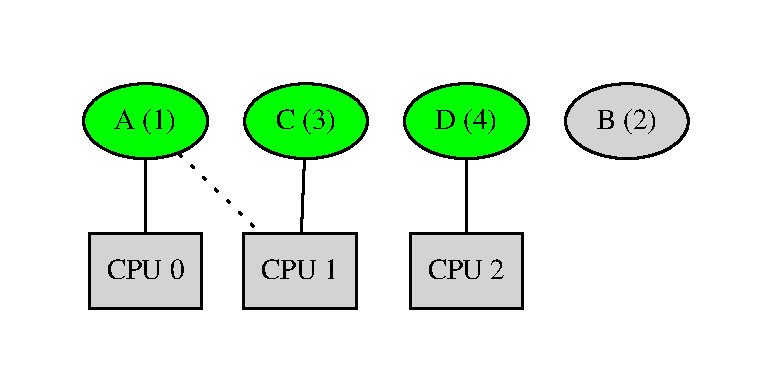
\includegraphics[width=\textwidth,height=\textheight/2,keepaspectratio=true]{dot_inline_dotgraph_2}}
\end{DoxyImageNoCaption}


At time t=2, Task B arrives and for an operating system that does not implement the Strong A\+PA scheduler (like Linux), the system looks like the following\+: (Since Task B has only C\+PU 0 in its affinity, it cannot displace Task A from C\+PU 0 because Task A has higher priority than Task B\+:


\begin{DoxyImageNoCaption}
  \mbox{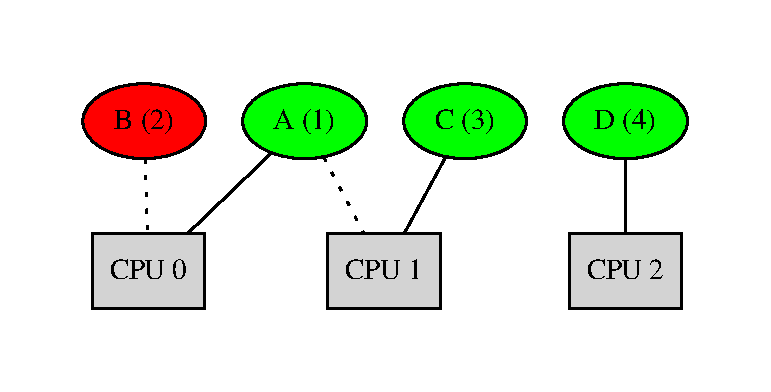
\includegraphics[width=\textwidth,height=\textheight/2,keepaspectratio=true]{dot_inline_dotgraph_3}}
\end{DoxyImageNoCaption}


Note here that the total sum of priorities of task scheduled is 1 + 3 + 4 = 8. On the arrival of Task B, a system that implements the Strong A\+PA scheduler would help task B in getting scheduled by searching for the lowest priority reachable task that could be preempted. This is done by recursively searching processors in the affinity set of Task B and for the task scheduled on those processor. So here Task A, which is scheduled on C\+PU 0 (the C\+PU in the affinity set of Task B) can also execute on C\+PU 1 since the latter C\+PU is also in Task A\textquotesingle{}s affinity set. Since C\+PU 1 has task C executing on it, which has a lower priority ( 3 $>$ 2) than Task B, preempting Task C to schedule Task A on C\+PU 1 and Task B on C\+PU 0 would result in the system executing tasks with total priority\+: 1 + 2 + 4 = 7 which is better than the previous case. So, for a system that implements the Strong A\+PA scheduler, at time t=2 the system would like\+:


\begin{DoxyImageNoCaption}
  \mbox{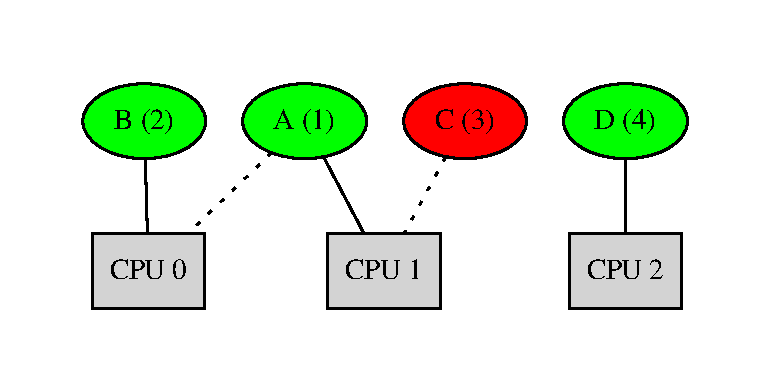
\includegraphics[width=\textwidth,height=\textheight/2,keepaspectratio=true]{dot_inline_dotgraph_4}}
\end{DoxyImageNoCaption}


The idea of this concept came from the problem of finding the M\+VM (Maximum Vertex Matching) where the priorities of task are encoded as weight of the vertices and the graph is a bi-\/partite graph that maps tasks to processor. This is similar to Caron et al.\+’s work that addresses a conceptually equivalent problem but in the different context of assigning employees with varying skill sets to open positions in order of seniority.

This is a very interesting topic and I would encourage you to learn more about the exact algorithms for scheduling a task on the event of task arrival/departure and the references to M\+VM problem by reading the following paper\+:

\mbox{[}1\mbox{]} Cerqueira, Felipe \& Gujarati, Arpan \& Brandenburg, Bjorn. (2015). Linux\textquotesingle{}s Processor Affinity A\+PI, Refined\+: Shifting Real-\/\+Time Tasks Towards Higher Schedulability. Proceedings -\/ Real-\/\+Time Systems Symposium. 2015. 249-\/259. 10.\+1109/\+R\+T\+SS.2014.\+29

Link to P\+DF version of paper\+:

\href{https://people.mpi-sws.org/~bbb/papers/pdf/rtss14f.pdf}{\tt https\+://people.\+mpi-\/sws.\+org/$\sim$bbb/papers/pdf/rtss14f.\+pdf} 